\section{Commande du robot}
\label{sec:control}

\subsection{Informatique distribuée}
\label{sub:distributed}

Les programmes développés nécessitent l'utilisation de plusieurs ordinateurs qui vont réaliser des tâches distinctes.
Le robot embarque deux ordinateurs, un double-coeur cadencé à 2.0GHz, et un simple-coeur à 1.8GHz fonctionnant avec un système d'exploitation temps réel.
Nous avons vu que l'algorithme RRT nécessite énormément de puissance, le premier ordinateur lui sera donc entièrement destiné.
Le second servira uniquement pour le contrôle comme nous le verrons dans le paragraphe \ref{sub:sot}.

D'autre part un ordinateur distant fonctionnant sous Windows assurera la localisation du robot et des différents obstacles (cf.~\ref{sub:env}), envoyant sur le réseau leurs positions à une fréquence de 200Hz. Afin de rendre le robot autonome cet ordinateur sera, dans le cadre d'un autre projet, supprimé et les calculs se feront directement sur le robot à partir des caméras embarquées.

Enfin un quatrième ordinateur sert de console, c'est à partir de celui-ci que l'on assure le démarrage des manipulations avec l'utilisation d'OpenHRP\footnote{Logiciel de contrôle du robot HRP, fourni par General Robotix.}. On peut également l'utiliser en tant que \emph{viewer} afin d'avoir un retour sur les positions des obstacles et des pas planifiés par le robot.

Afin de pouvoir faire marcher le robot, il faut que toutes les informations soient synchronisées, pour cela nous utiliserons une synchronisation universelle et nous récupérons la valeur du temps avec la librairie \emph{boost}.

%% \begin{figure}[h]
%% \begin{center}
%% 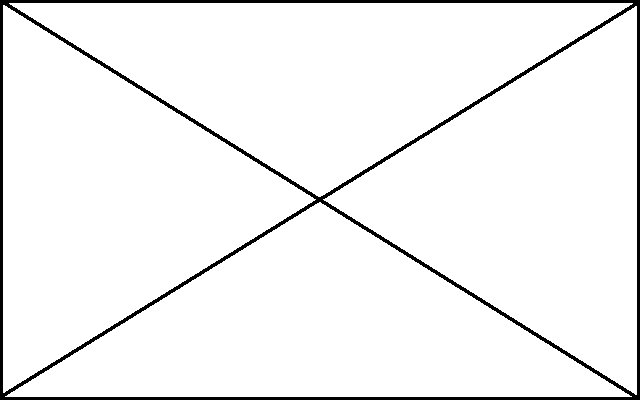
\includegraphics[width=10.0cm]{images/vide.jpg}
%% \caption{Organisation des différents ordinateurs utilisés lors de la replannification.}
%% \label{fig:PC}
%% \end{center}
%% \end{figure}

\subsection{Serveur de communication}
\label{sub:corba}

Il est primordial d'assurer une bonne communication entre les différents ordinateurs utilisés. Nous avons alors mis en place un serveur \emph{Corba} sur le PC temps-réel. Cette entité \emph{python} permet de connecter des flux de données entre eux. 

Chaque programme va pouvoir venir lire librement la valeur d'une variable circulant dans un flux si celui-ci est \emph{pluggé}. Ils pourront mettre à jour les différentes variables afin de commander le robot, ou simplement d'afficher les résultats obtenus. Les flux sont représentés dans la figure~\ref{fig:corba}, tous les flux allant vers le \emph{viewer} sont facultatifs, ils ne participent pas à la marche du robot.

\begin{figure}[h]
\begin{center}
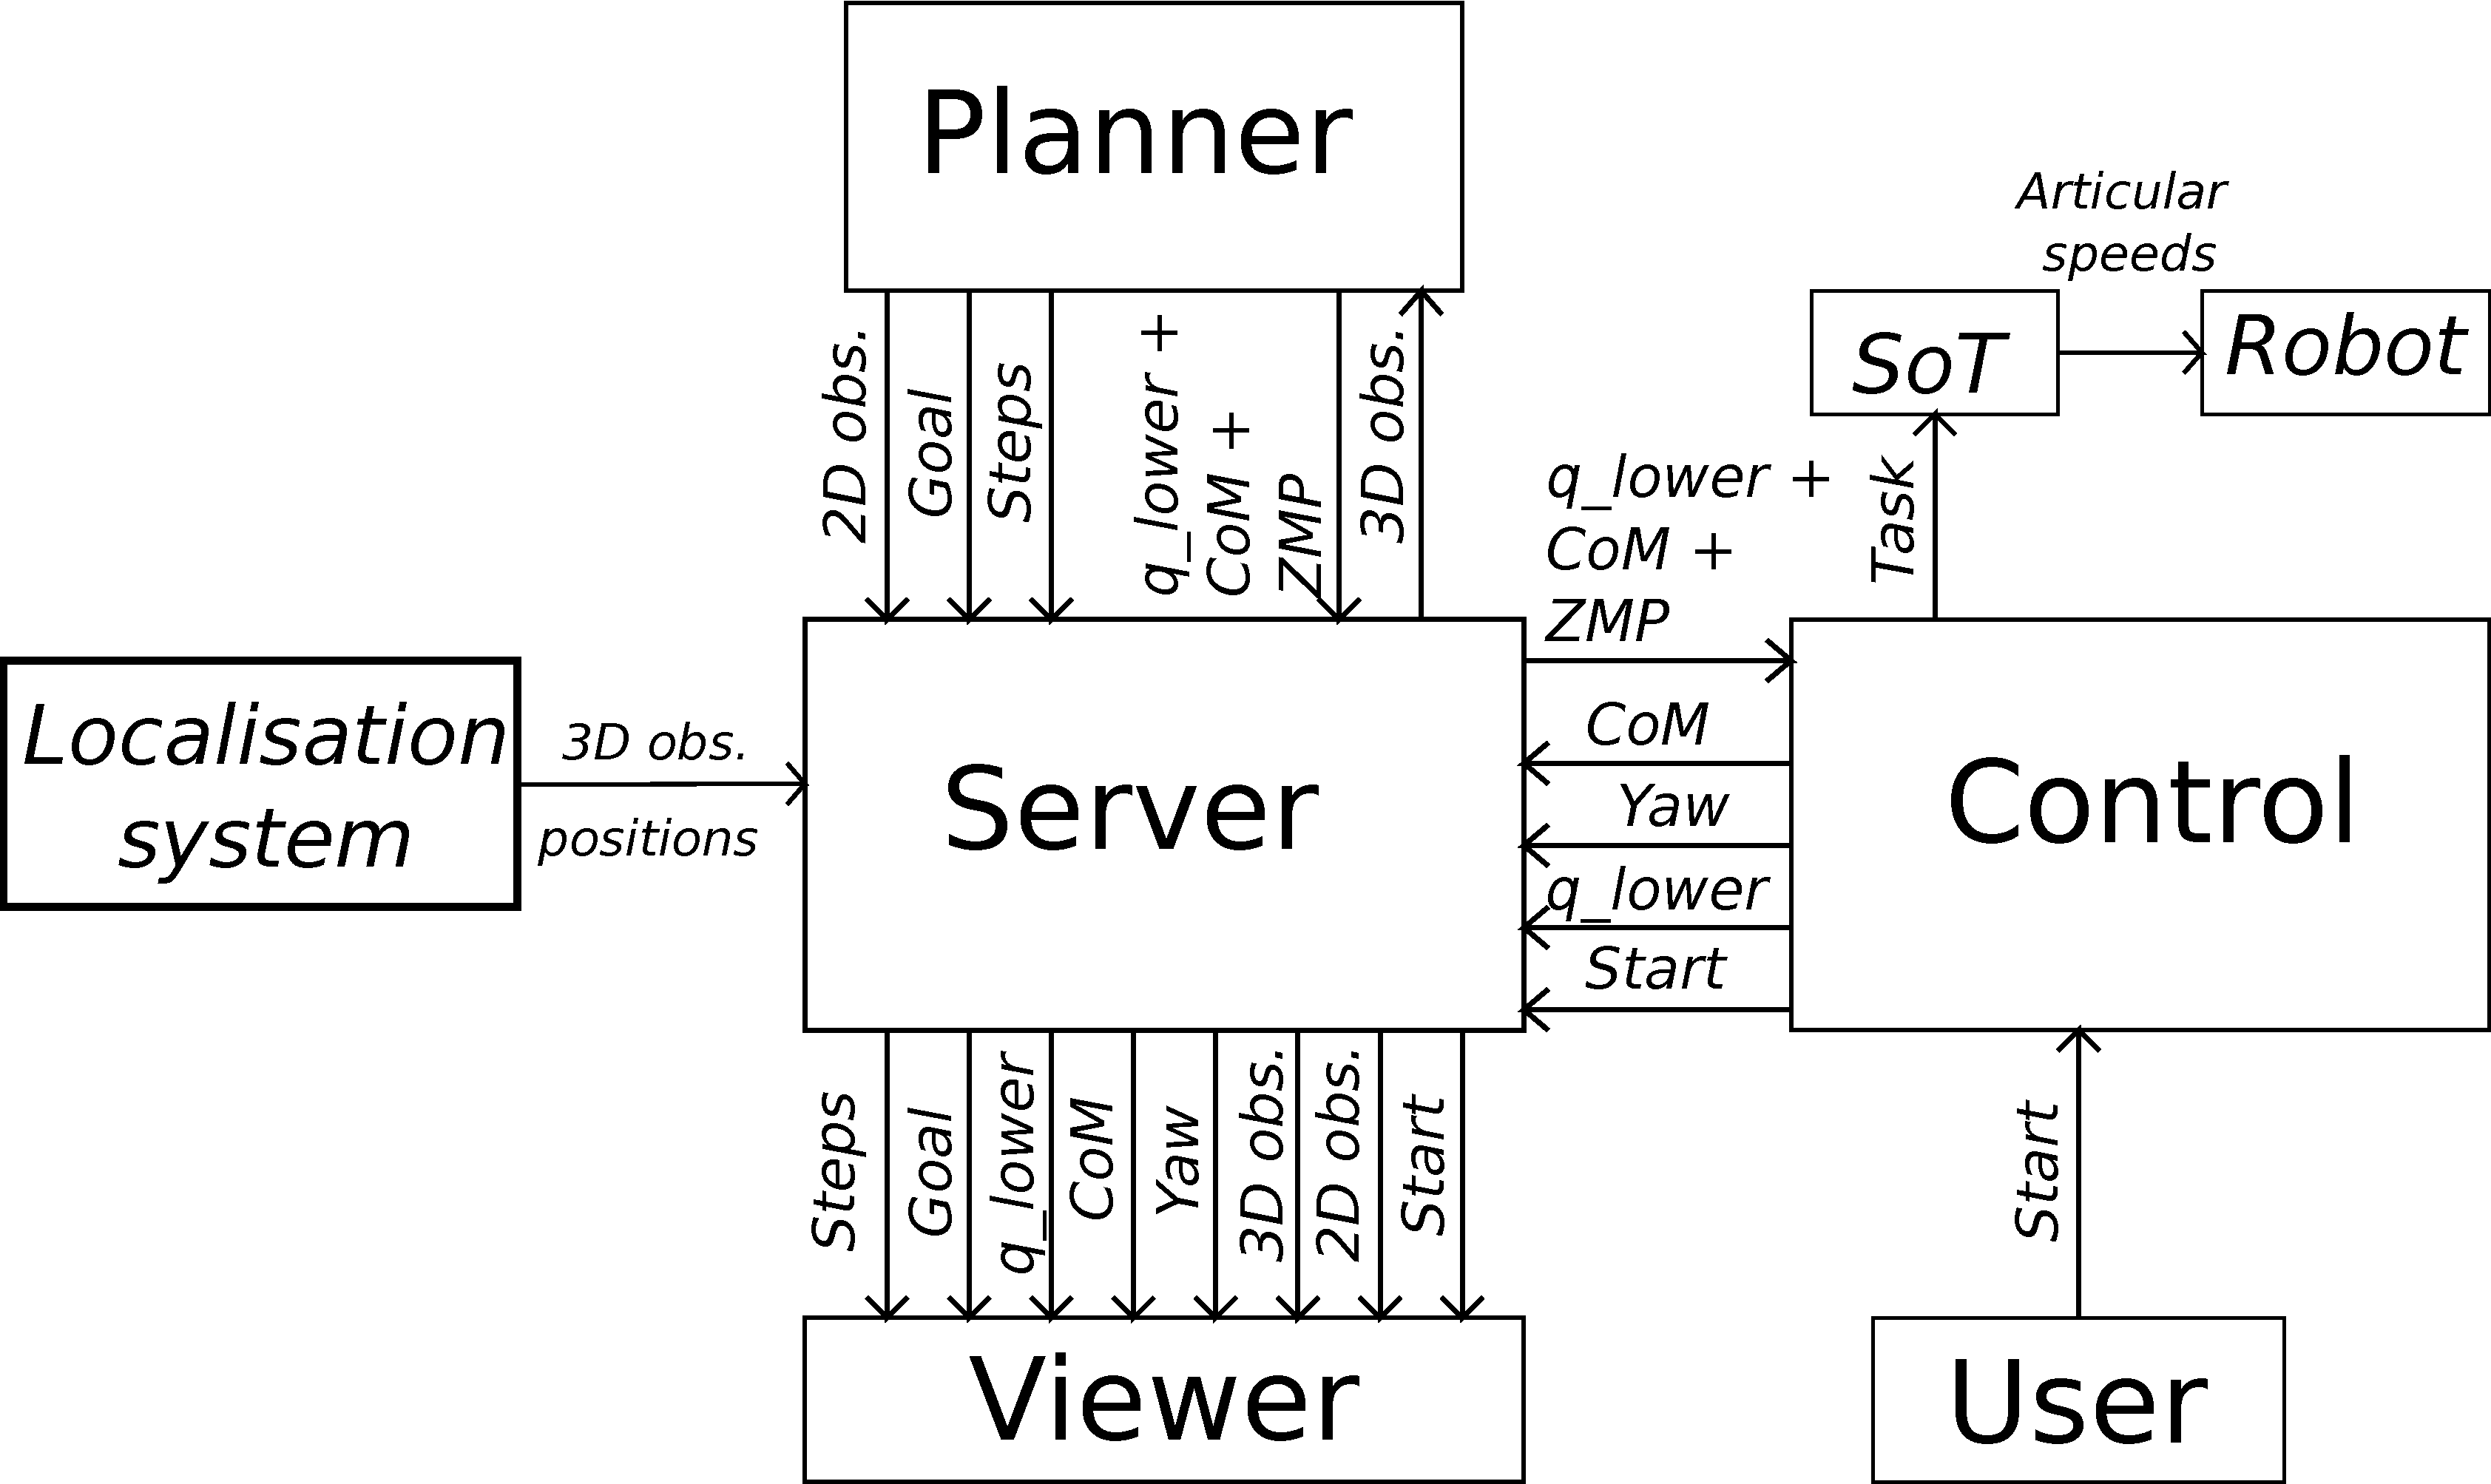
\includegraphics[width=12.0cm]{images/corba.png}
\caption{Flux d'informations transmis via le serveur Corba.}
\label{fig:corba}
\end{center}
\end{figure}

En \emph{pluggant} sur ce serveur une entité permettant la mise en mémoire de données, on peut sauvegarder la totalité des informations transmises ce qui permet un \emph{débogage} rapide en cas d'anomalies.


\subsection{Valeurs articulaires}
\label{sub:valeurs}

Le \emph{planner} créer les positions du \emph{waist} (bassin) et des pieds tout au long de la trajectoire lors du \emph{smoothing}. A partir de ses données on peut facilement retrouver les valeurs articulaires du robot à l'aide d'une invertion cinématique.
On obtient alors un vecteur contenant toutes les valeurs articulaires du robot pour un chemin donné. En choisissant comme longueur de chemin, la durée d'un pas, on a des petits vecteurs, environ 5000 \emph{doubles}, ce qui représente environ 250 kilo-octects de données qui sont facilement transférables par réseau vers l'ordinateur qui gère le contrôle. La figure~\ref{fig:message} est un exemple d'utilisation de ces \emph{messages} qui circulent en permanence sur le réseau, on peut voir que le message 3 vient écraser les valeurs précédément reçues via le message 2.

\begin{figure}[h]
\begin{center}
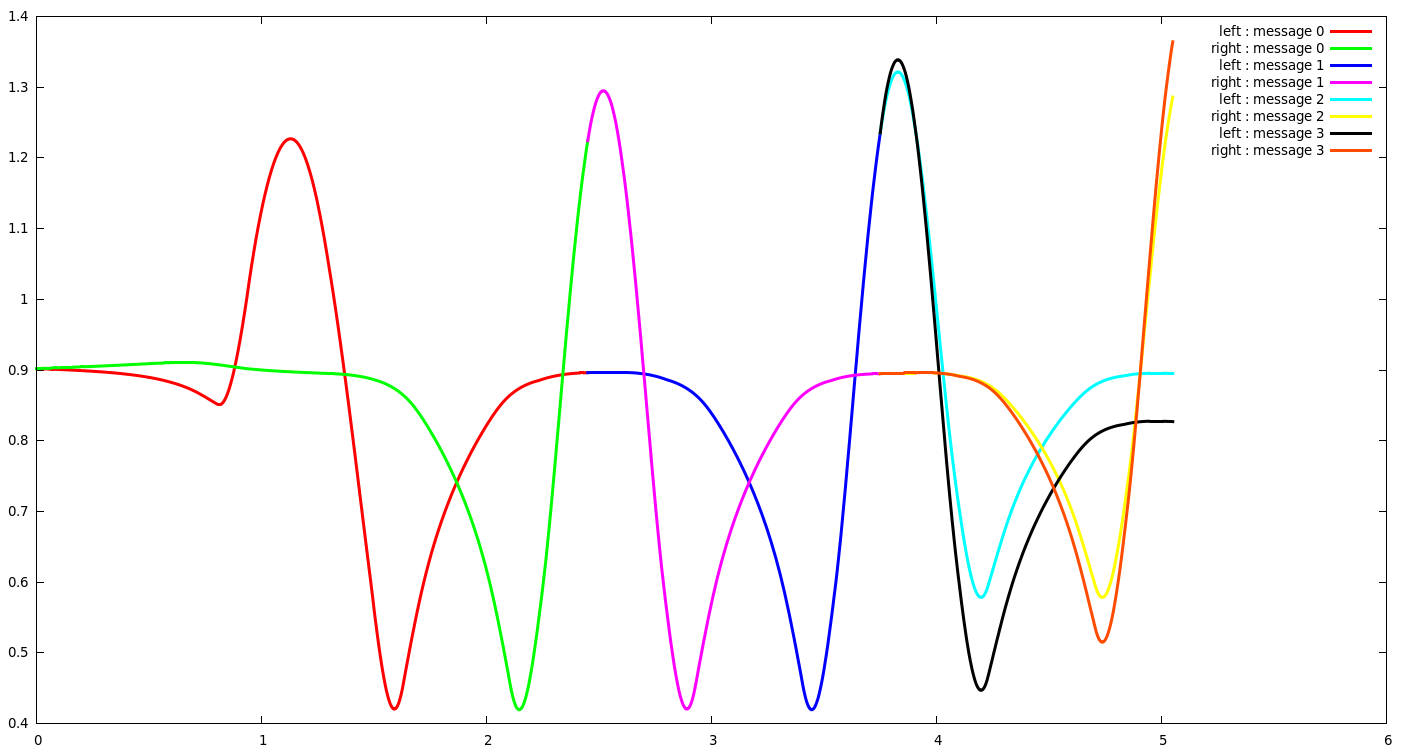
\includegraphics[width=15.0cm]{images/messages.png}
\caption{Exemple d'une série de messages contenant les valeurs articulaires envoyées via Corba. Ici seules les articulations des genoux sont tracées, chaque couleur représente un message différent ou une articulation différente.}
\label{fig:message}
\end{center}
\end{figure}

Il convient dans ce genre de transfert de vérifier qu'aucun message n'a été perdu lors de la communication, afin d'éviter des valeurs aberrantes sur les consignes des moteurs. Pour cela chaque message est muni d'un identifiant, et de la longueur totale de la trajectoire. Ceci permet, à la réception d'un message, de constater si le message portant l'identifiant précédent à bien été reçu. L'utilisation de la longueur de la trajectoire permet de vérifier que le dernier message a également bien été réceptionné. Si un seul message a été perdu pendant les communications, un processus d'arrêt d'urgence immobilise le robot afin d'éviter des mouvements dangereux.


\subsection{Application des consignes}
\label{sub:sot}

Une fois les données sur les valeurs articulaires des jambes receptionnées, il faut appliquer les consignes au niveau des moteurs du robot.
Une notion de stabilité apparait quand on travaille avec  des robots humanoïdes, il ne faut pas que le robot tombe si il est légèrement perturbé. Pour celà on doit déplacer le \emph{ZMP}~\cite{Kajita03bipedwalking} (zero-moment-point) et le centre de masse (\emph{CoM}) du robot afin de les placer au niveau de ceux planifiés.
Nous imposons des valeurs fixes au niveau des bras du robots afin de pouvoir calculer plus facilement le CoM.
%Cependant un robot à 36 degrés de liberté n'est pas aussi simple à commander qu'un robot industriel. 

On peut donc résumer ces différentes contraintes sous forme de tâches distinctes, qui vont chacune commander une partie du robot à 36 degrés de liberté.
Afin que le robot puisse être multi-tâches, une structure de piles-de-tâches (\emph{Stack~of~Task}~\cite{mansard:ieeetro:2007}) a été mise en place sur HRP-2, elle contient les équations concerant chacune des tâches ainsi que leurs gains et leurs priorités relatives.

Un \emph{solver} va tenter toutes les $5ms$ de résoudre au mieux les différentes équations qui contraignent le robot. La figure~\ref{fig:sot} représente les différentes tâches appliquées dans la SoT. Ici le ZMP est utilisé par le stabilisateur interne du robot, il ne passera donc pas par la SoT.

\begin{figure}[h]
\begin{center}
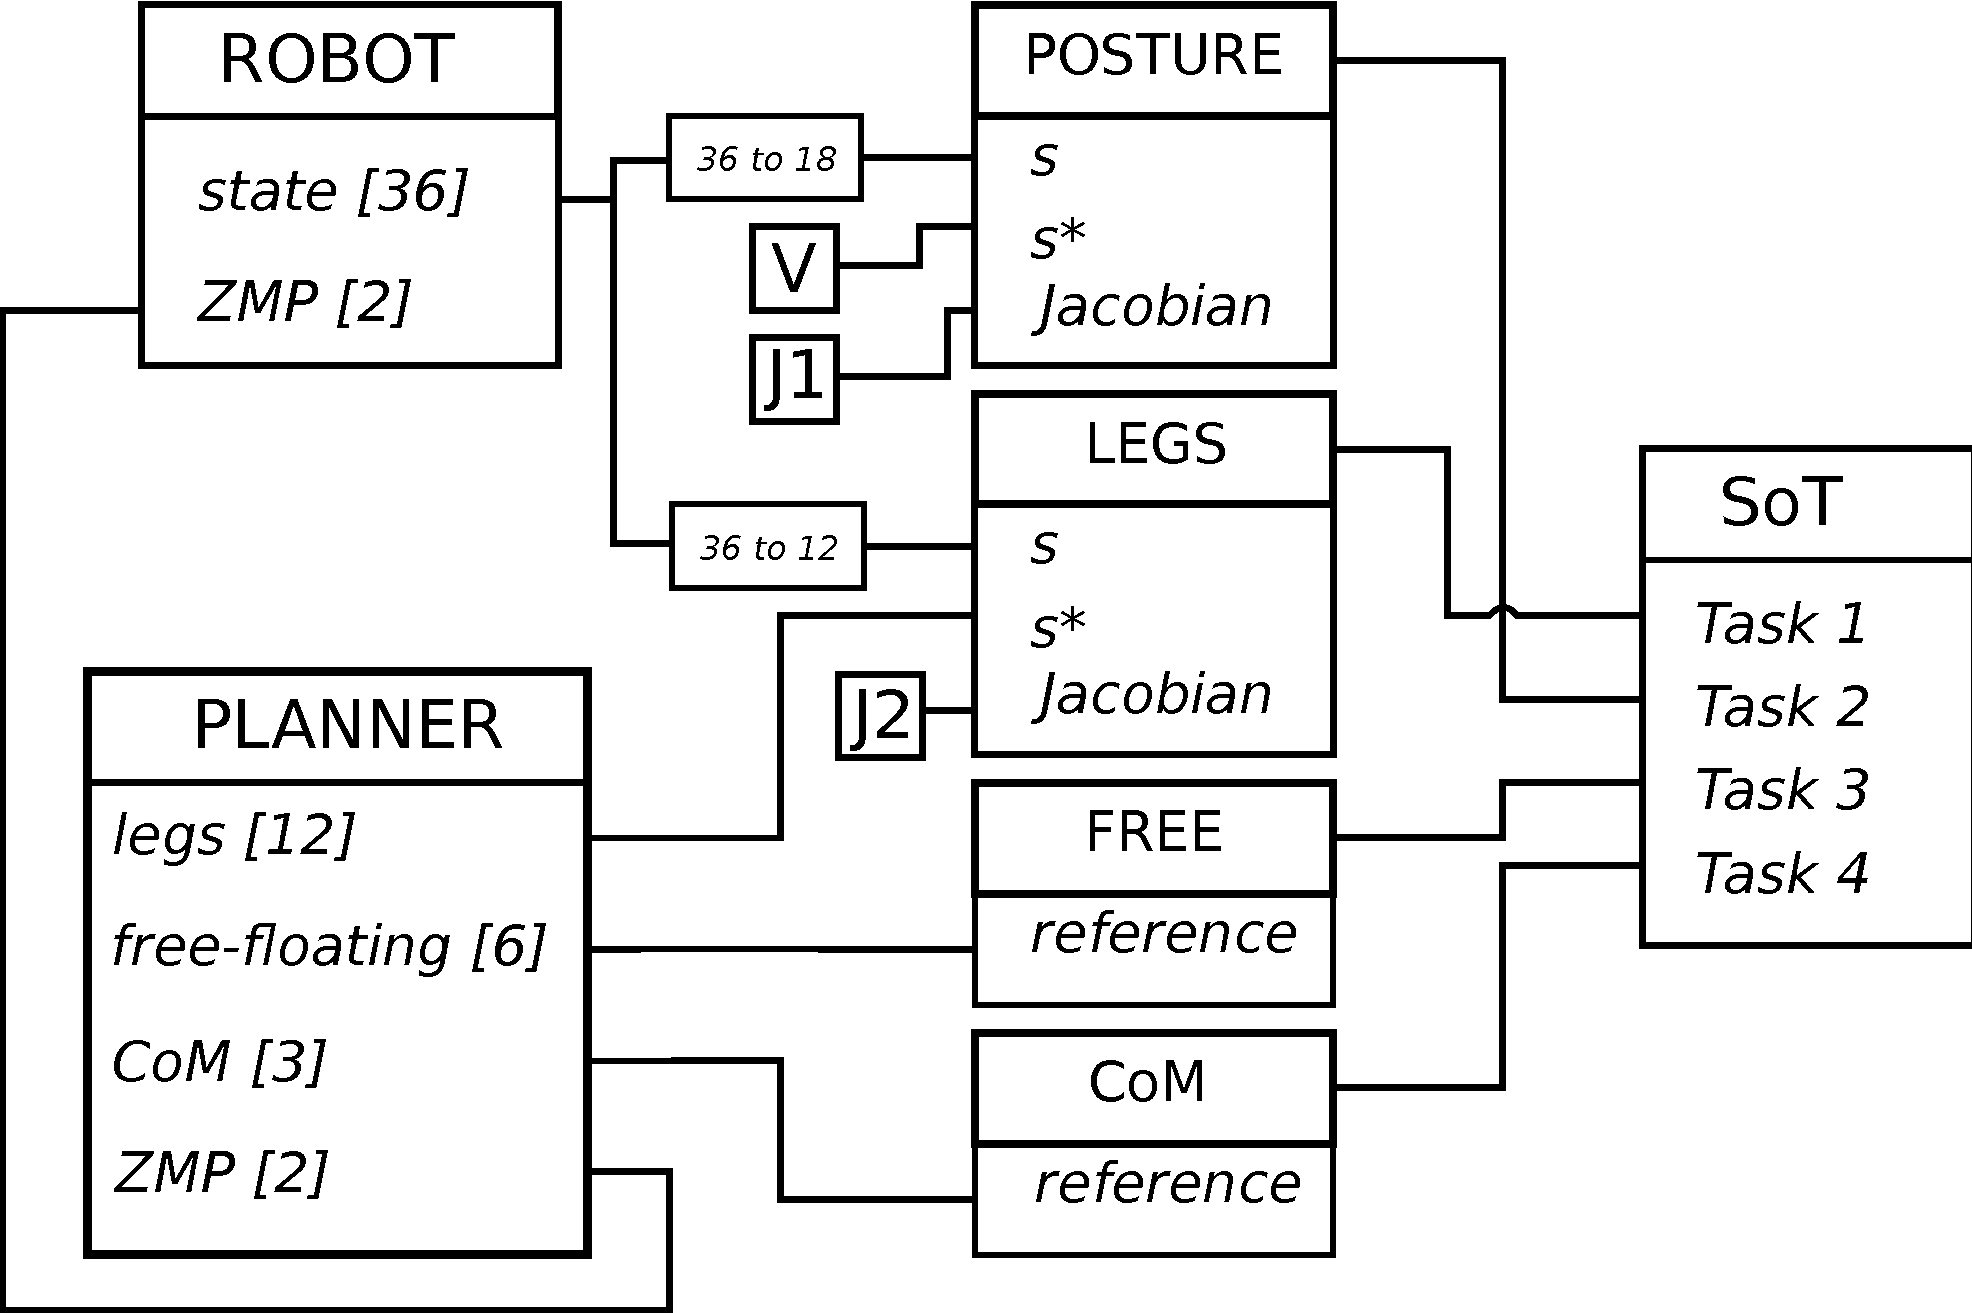
\includegraphics[width=9.0cm]{images/SoT.png}
\caption{Tâches présentes dans la \emph{Stack of Task}. $J1$ et $J2$ représentent les jacobiennes liées aux tâches. $V$ est un vecteur de valeurs fixes.}
\label{fig:sot}
\end{center}
\end{figure}

Dans notre cas la SoT n'a pas vraiment d'utilité car nous n'utilisons pas toutes les capacités du robot (les bras restant fixes). Cependant nous pourrions dans le futur utiliser des nouvelles tâches afin de manipuler des objets tout en marchant, il suffirait uniquement de modifier la tâche de posture, les jambes continueraient d'exécuter les consignes reçues.

